\documentclass[russian,utf8,a1paper,nostitching,simple]{eskdgraph}
\usepackage[T2A]{fontenc}
\usepackage{pscyr}
\usepackage{tikz}
\usepackage{color}

\newcommand{\No}{\textnumero}

\ESKDunitName{Алгоритм оптического распознавания числовых данных}
\ESKDsignature{ГУИР.000000.004 ПЛ}
\ESKDletter{}{Т}{}
\ESKDauthor{Будный}
\ESKDchecker{Сальников}
\ESKDcolumnXIfIII{Лаппо}
\ESKDnormContr{Протченко}
\ESKDapprovedBy{Навроцкий}
\ESKDgroup{ИТАС, гр. 120602}

\begin{document}

\ESKDthisStyle{empty}
\begin{ESKDdrawing}
  \centering
  {\fontsize{50}{60}\selectfont Алгоритм оптического распознавания числовых данных}

  \vspace{2cm}
  \centering
  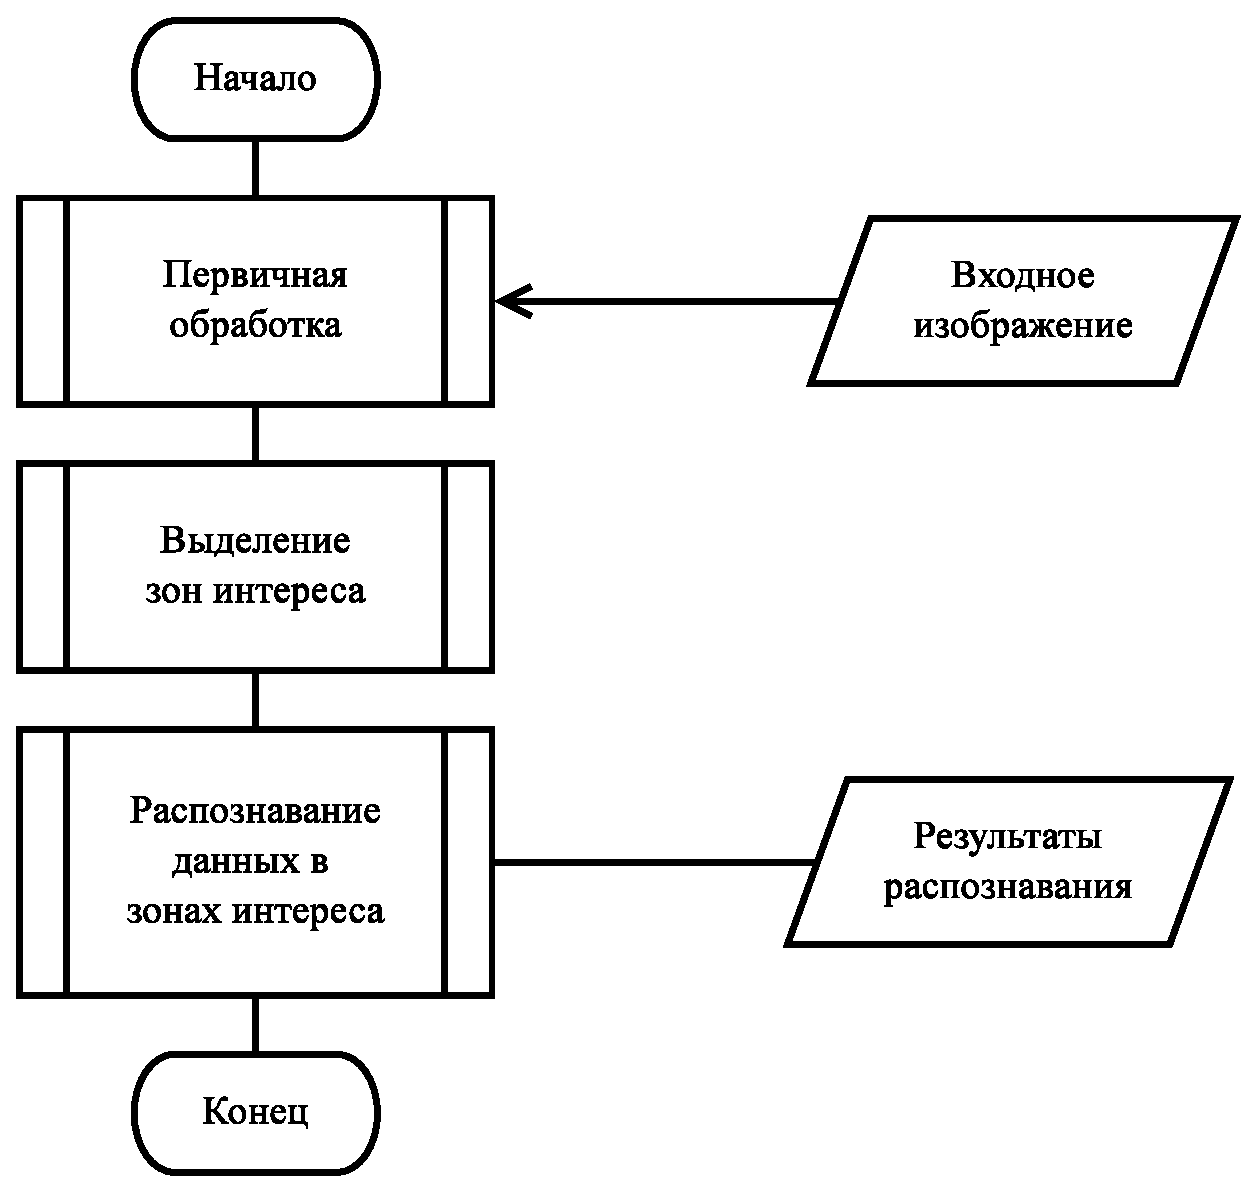
\includegraphics[height=20cm]{fig/design_algorithm_basic.eps}

    % \vspace{4cm}
    % \centering
    % \ESKDfontX{Классы обработки пользовательского ввода} \\
    % \vspace{2cm}
    % \centering
    % 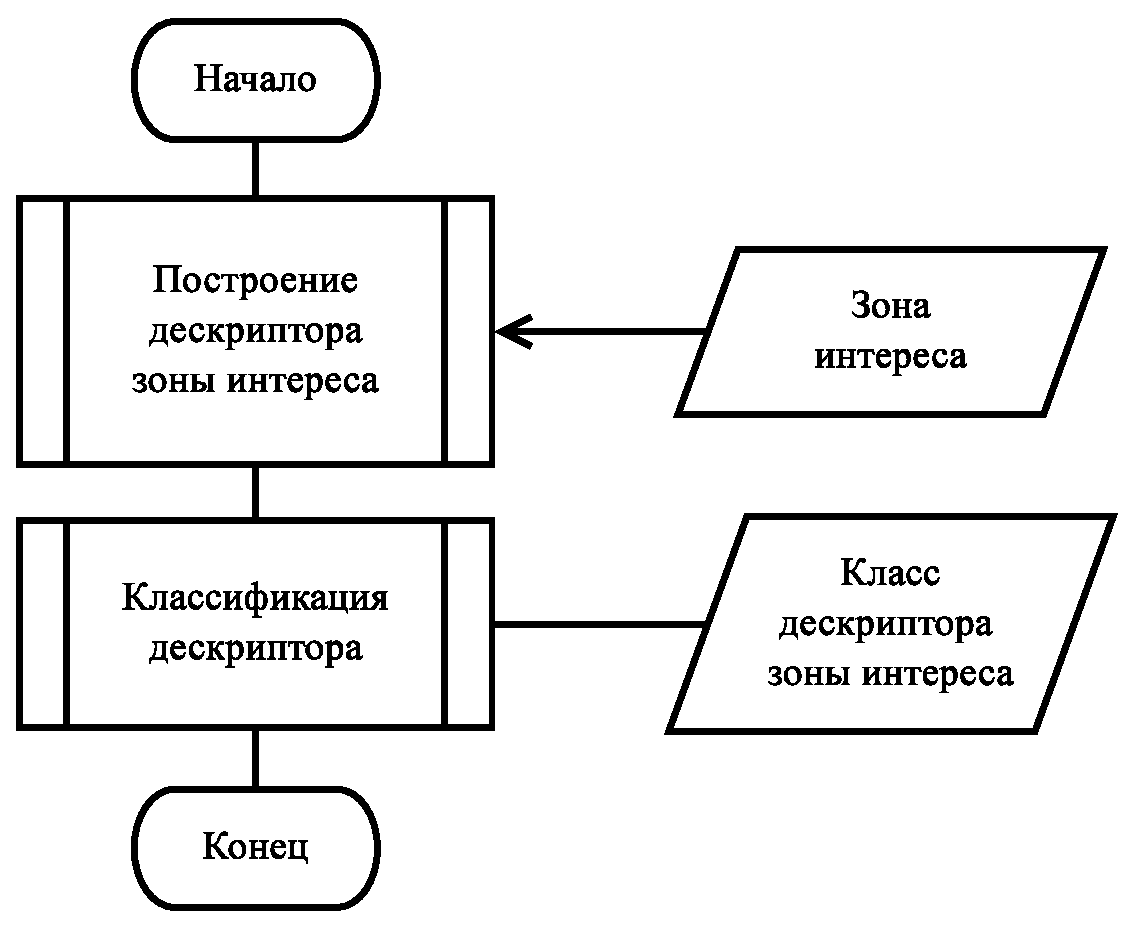
\includegraphics[height=20cm]{fig/design_algorithm_recognition.eps}
\end{ESKDdrawing}

\setcounter{page}{1}
\ESKDthisStyle{formI}
\begin{ESKDdrawing}
\end{ESKDdrawing}

\end{document}
